% Compile from the slides directory with: xelatex presentation.tex
\documentclass[aspectratio=169,11pt]{beamer}
\usetheme{Madrid}
\usecolortheme{default}
\usepackage{graphicx}
\usepackage{booktabs}
\usepackage{array}
\usepackage{xcolor}
\usepackage{tikz}
\usetikzlibrary{arrows.meta}
\usepackage{xepersian}
\settextfont{Tahoma}
\setlatintextfont{Arial}
\definecolor{navy}{HTML}{16324F}
\definecolor{teal}{HTML}{087E8B}
\definecolor{amber}{HTML}{D18B22}
\setbeamercolor{structure}{fg=teal}
\setbeamercolor{frametitle}{fg=white,bg=navy}
\setbeamercolor{title}{fg=white,bg=navy}
\setbeamercolor{block title}{fg=white,bg=teal}
\setbeamercolor{block body}{bg=teal!7}
\setbeamercolor{alerted text}{fg=amber}
\setbeamercolor{footline}{fg=white,bg=navy}
\setbeamertemplate{navigation symbols}{}
\setbeamertemplate{footline}[frame number]
\setbeamertemplate{itemize item}{\color{teal}$\blacktriangleright$}
\setbeamertemplate{itemize subitem}{\color{teal}$\bullet$}
\newcommand{\key}[1]{\textcolor{teal}{\textbf{#1}}}
\newcommand{\eng}[1]{\lr{#1}}
\newcommand{\smallsource}[1]{{\tiny\color{gray}منبع شکل: \lr{\detokenize{#1}}}}

\title{تشخیص و مکان‌یابی نشت در شبکهٔ آب \eng{L-Town}}
\subtitle{از شبیه‌سازی هیدرولیکی تا دو شبکهٔ \eng{MLP}}
\author{ارائهٔ پروژهٔ یادگیری عمیق}
\date{}

\begin{document}

\begin{frame}
  \titlepage
  \vspace{-1em}
  \begin{center}\small نمونهٔ اولیهٔ ارائه؛ اعداد از \eng{report.md} و خروجی اجرای کد گرفته شده‌اند.\end{center}
\end{frame}

\begin{frame}{پرسش پروژه و پاسخ ما}
  \begin{block}{دو پرسش عملی}
  آیا در شبکه نشت فعال است؟ اگر بله، جست‌وجو را از کدام گروهِ لوله‌ها شروع کنیم؟
  \end{block}
  \begin{itemize}
  \item \key{آشکارساز} از دادهٔ زمانی حسگرها احتمال نشت می‌دهد.
  \item \key{مکان‌یاب} فقط هنگام هشدار، ۲۰ خوشهٔ لوله را به ترتیب احتمال پیشنهاد می‌کند.
  \item خوشه یعنی لوله‌هایی که نشتشان در ۳۳ حسگر فشار، اثر مشابه دارد؛ خروجی، یک لولهٔ دقیق نیست.
  \end{itemize}
  \vspace{0.3em}
  \begin{center}\color{navy}\large دادهٔ حسگر $\longrightarrow$ احتمال نشت $\longrightarrow$ هشدار $\longrightarrow$ فهرست خوشه‌ها\end{center}
\end{frame}

\begin{frame}{داده‌هایی که واقعاً در اختیار داریم}
  \begin{itemize}
  \item شبکه: \key{۷۸۲ گره}، \key{۹۰۵ لوله} و فقط \key{۳۳ حسگر فشار}.
  \item دادهٔ ۲۰۱۸: هر ۵ دقیقه یک ردیف؛ در کل \key{۱۰۵٬۱۲۰ ردیف}.
  \item هر ردیف: ۳ جریان ورودی، تراز یک مخزن و مصرف ۸۲ کنتور خانگی \eng{AMR}، در کنار فشارها.
  \item برچسب واقعی: \key{۲۰ رخداد نشت}؛ ۱۳ نشت ناگهانی و ۷ نشت تدریجی.
  \item نشت‌ها طولانی‌اند و بعضی هم‌زمان رخ می‌دهند؛ بنابراین ردیف‌های زمانی مستقل نیستند.
  \end{itemize}
  \begin{block}{چالش اصلی}
  فشار به مصرف روزانه و وضعیت مخزن هم وابسته است؛ افت فشار به‌تنهایی نشانهٔ قطعی نشت نیست.
  \end{block}
\end{frame}

\begin{frame}{نقشهٔ الگوریتم: از داده تا تصمیم}
  \begin{enumerate}
  \item مدل هیدرولیکی، اثر نشت در نقاط شبکه را روی حسگرها شبیه‌سازی می‌کند.
  \item لوله‌های با الگوی فشار مشابه به ۲۰ خوشه تقسیم می‌شوند.
  \item پیش‌پردازش، رفتار عادی فشار و جریان را یاد می‌گیرد و اختلاف مشاهده با انتظار را می‌سازد.
  \item \eng{MLP} اول احتمال نشت را تخمین می‌زند؛ میانگین سه‌ساعته و آستانه، هشدار را تعیین می‌کنند.
  \item \eng{MLP} دوم، هنگام هشدار، خوشه‌ها را برای جست‌وجو مرتب می‌کند.
  \end{enumerate}
  \vspace{0.5em}
  \begin{block}{مرز مهم}
  شبیه‌ساز برای ساخت امضا و نمونهٔ آموزشی است؛ هنگام پیش‌بینی، ورودی مدل فقط دادهٔ حسگرهاست.
  \end{block}
\end{frame}

\begin{frame}{مدل هیدرولیکی چگونه به کار رفت؟}
  \begin{itemize}
  \item با \eng{WNTR/EPANET} برای هر گره، یک نشت نمونه شبیه‌سازی شد؛ فشار ۳۳ حسگر با حالت بدون نشت مقایسه شد.
  \item هر شبیه‌سازی ۴۸ ساعت بود؛ روز اول برای حذف اثر گذرای مخزن کنار رفت.
  \item نتیجهٔ هر محل، یک \key{امضای فشار} است: الگوی افت در ۳۳ حسگر.
  \item برای نشت وسط لوله، امضای دو سر لوله میانگین گرفته شد؛ این تقریب در ۱۰ لوله جداگانه بررسی شد.
  \item اندازهٔ نشت با تقریب مربع قطر تغییر داده شد؛ یک گره استثنای آشکار داشت و این محدودیت ثبت شد.
  \end{itemize}
  \begin{block}{کنترل اولیهٔ واحدها}
  برای نشت ۱٫۵ سانتی‌متری در \eng{n500}، افزایش جریانِ شبیه‌سازی‌شده ۱۵٫۲۶ مترمکعب‌برساعت بود؛ مقدار راهنما حدود ۱۵ است.
  \end{block}
\end{frame}

\begin{frame}{چرا خروجی مکان‌یاب «خوشه» است؟}
  \begin{columns}[T,onlytextwidth]
  \begin{column}{0.55\textwidth}
  \begin{itemize}
  \item اثر نشتِ بعضی لوله‌ها روی حسگرهای محدود، تقریباً یکسان است.
  \item امضاها را با روش \eng{Ward} بر اساس شکل افت فشار گروه‌بندی کردیم.
  \item \key{۲۰ خوشه} انتخاب شد: ۹۰۰ لولهٔ قابل مشاهده و ۵ لولهٔ بسیار کم‌اثر.
  \item ۲۰ نشت واقعی فقط در ۱۱ خوشه رخ داده‌اند؛ برای بقیه، نمونهٔ مصنوعی لازم شد.
  \end{itemize}
  \end{column}
  \begin{column}{0.43\textwidth}
  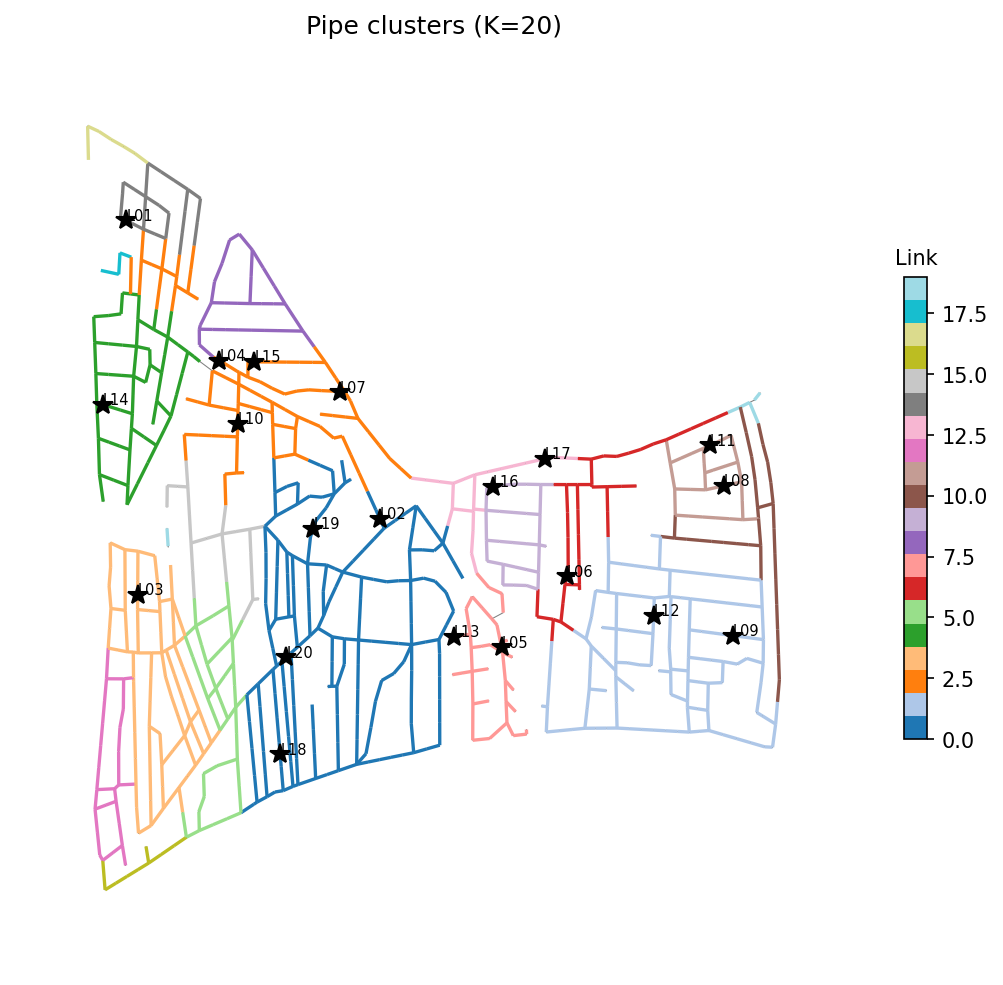
\includegraphics[width=0.92\linewidth]{../outputs/part1/p1_cluster_map.png}
  \smallsource{outputs/part1/p1_cluster_map.png}
  \end{column}
  \end{columns}
\end{frame}

\begin{frame}{تقسیم زمانی و جلوگیری از نشت اطلاعات}
  \begin{center}
  \begin{tikzpicture}[
    every node/.style={draw=teal,rounded corners=3pt,align=center,text width=2.45cm,minimum height=1.15cm,font=\footnotesize},
    x=1cm,y=1cm]
    \node[fill=teal!10] (b3) at (1.5,0) {بلوک ۳\\۱۱ سپتامبر تا پایان سال};
    \node[fill=teal!10] (b2) at (4.4,0) {بلوک ۲\\۱۴ ژوئن تا ۱۱ سپتامبر};
    \node[fill=amber!20,draw=amber] (b1) at (7.3,0) {\textbf{بلوک ۱: ارزیابی}\\۱۵ مارس تا ۱۴ ژوئن};
    \node[fill=teal!10] (b0) at (10.2,0) {بلوک ۰\\۱ ژانویه تا ۱۵ مارس};
    \draw[-{Latex[length=2mm]},thick,navy] (b0.west) -- (b1.east);
    \draw[-{Latex[length=2mm]},thick,navy] (b1.west) -- (b2.east);
    \draw[-{Latex[length=2mm]},thick,navy] (b2.west) -- (b3.east);
  \end{tikzpicture}
  \end{center}
  \vspace{0.2em}
  \small در نوبتِ نشان‌داده‌شده، بلوک ۱ برای ارزیابی است و سه بلوک دیگر برای آموزش‌اند.
  \begin{itemize}
  \item مرزها در فاصله‌های بدون نشت‌اند؛ ردیف‌های آموزشیِ تا ۲۴ ساعت کنار بلوک ارزیابی حذف می‌شوند.
  \item هر بلوک یک بار ارزیابی می‌شود؛ کنار هم گذاشتن چهار خروجی، پیش‌بینی \eng{OOF} سال ۲۰۱۸ را می‌سازد.
  \end{itemize}
  \begin{block}{چرا تقسیم تصادفی ردیف‌ها مناسب نیست؟}
  یک نشت ممکن است هفته‌ها ادامه داشته باشد؛ تقسیم تصادفی می‌تواند همان رخداد را هم در آموزش و هم در ارزیابی بگذارد.
  \end{block}
\end{frame}

\begin{frame}{در هر نوبت ارزیابی، کد چه می‌کند؟}
  \begin{enumerate}
  \item سه بلوکِ آموزش را انتخاب می‌کند و ردیف‌های نزدیک مرز ارزیابی را کنار می‌گذارد.
  \item مدلِ «رفتار عادی» و مقیاس‌بندی اختلاف‌ها را فقط روی دادهٔ مجازِ آموزش برازش می‌کند.
  \item نشت‌های مصنوعی را فقط به همان بخش آموزش می‌افزاید و \eng{MLP} را آموزش می‌دهد.
  \item پیش‌بینیِ بلوک کنارگذاشته‌شده را ذخیره می‌کند؛ این بلوک در آموزش آن نوبت دیده نشده است.
  \end{enumerate}
  \begin{block}{خروجی خارج از آموزش یعنی چه؟}
  این چهار نوبت، برای همهٔ سال یک پیش‌بینی می‌دهند؛ اما پیش‌بینیِ هر ردیف را مدلی ساخته که آن ردیف را در آموزش ندیده است. به آن \eng{out-of-fold (OOF)} می‌گوییم.
  \end{block}
  \small\color{gray}چهار مدل این مرحله برای مقایسه‌اند؛ پس از انتخاب طراحی، مدلِ تحویل‌دادنی با دادهٔ مجازِ کل سال آموزش می‌بیند.
\end{frame}

\begin{frame}{پیش‌پردازش: «رفتار عادی» را از نشت جدا کنیم}
  \begin{enumerate}
  \item از فشارها، جریان ورودی، مصرف \eng{AMR} و تراز مخزن، میانگین یک‌ساعتهٔ گذشته را می‌گیریم.
  \item روی ساعت‌های بدون نشتِ \key{آموزش}، مدلی ساده برای فشار و جریان مورد انتظار می‌سازیم.
  \item ورودی این مدل عادی: ساعت روز، روز کاری/آخر هفته، مصرف کل \eng{AMR}، تراز و تغییر تراز مخزن.
  \item اختلاف \key{فشار مشاهده‌شده و مورد انتظار} برای ۳۳ حسگر و اختلاف \key{جریان ورودی و مورد انتظار} یک بردار ۳۴تایی می‌سازد.
  \end{enumerate}
  \begin{block}{دلیل استفاده از \eng{AMR} و مخزن}
  کاهش فشار می‌تواند از افزایش مصرف یا تغییر ذخیرهٔ مخزن باشد؛ مدل عادی کمک می‌کند اثر این تغییرها با نشت اشتباه نشود.
  \end{block}
\end{frame}

\begin{frame}{ورودی آشکارساز دقیقاً چیست؟}
  \begin{itemize}
  \item \key{۳۴ اختلاف اندازه‌گیری‌شده در زمان فعلی}: ۳۳ اختلاف فشار و یک اختلاف جریان.
  \item همان ۳۴ عدد برای پنج زمانِ پیش از آن، با فاصلهٔ یک ساعت: در مجموع \key{۲۰۴ عدد}.
  \item ۵ ویژگی زمانی برای ساعت روز، روز هفته و آخر هفته افزوده می‌شود.
  \end{itemize}
  \begin{center}\Large\color{navy}$6\times 34+5=\mathbf{209}$\end{center}
  \begin{block}{نکتهٔ اجرایی}
  همهٔ میانگین‌ها و پنجره‌ها فقط از زمان فعلی و گذشته استفاده می‌کنند. در آغاز فایل، زمان‌های پیشینِ موجود نبودن با مقدار استانداردشدهٔ صفر پر می‌شوند.
  \end{block}
\end{frame}

\begin{frame}{یک مثال قدم‌به‌قدم از ورودی ۲۰۹تایی}
  \begin{block}{مرحلهٔ ۱: اختلاف فشار یک حسگر در ساعت ۱۰}
  مثال فرضی: میانگین فشار یک‌ساعتهٔ حسگر \eng{P1} برابر ۴۴٫۲ متر و مقدارِ مورد انتظارِ مدل عادی ۴۵٫۰ متر است؛ اختلاف آن‌ها \key{۰٫۸- متر} می‌شود. اگر انحراف معیارِ این اختلاف در آموزش ۰٫۴ متر باشد، ورودی استانداردشدهٔ این حسگر \key{۲-} است.
  \end{block}
  \begin{center}
  \begin{tikzpicture}[every node/.style={draw=teal,rounded corners=2pt,fill=teal!8,align=center,text width=1.5cm,minimum height=.85cm,font=\small},x=1cm]
    \node at (0.85,0) {ساعت ۵\\۳۴ عدد};
    \node at (2.65,0) {ساعت ۶\\۳۴ عدد};
    \node at (4.45,0) {ساعت ۷\\۳۴ عدد};
    \node at (6.25,0) {ساعت ۸\\۳۴ عدد};
    \node at (8.05,0) {ساعت ۹\\۳۴ عدد};
    \node[fill=amber!20,draw=amber] at (9.85,0) {ساعت ۱۰\\۳۴ عدد};
  \end{tikzpicture}
  \end{center}
  \begin{center}\color{navy}\large شش بردار ۳۴تایی = ۲۰۴ عدد؛ با ۵ ویژگیِ زمانِ ساعت ۱۰ $\longrightarrow$ \textbf{۲۰۹ ورودی}\end{center}
  \small\color{gray}در هر بردار: ۳۳ اختلاف فشار و یک اختلاف جریان ورودی و مورد انتظار؛ همهٔ مقدارها فقط از همان زمان و گذشته به دست می‌آیند.
\end{frame}

\begin{frame}{آموزش آشکارساز: معماری و هایپرپارامترها}
  \begin{center}\color{navy}\large ۲۰۹ ورودی $\longrightarrow$ ۱۲۸ نورون $\longrightarrow$ ۶۴ نورون $\longrightarrow$ احتمال نشت\end{center}
  \begin{itemize}
  \item هر لایهٔ پنهان: \eng{Linear → BatchNorm → ReLU → Dropout(0.2)}.
  \item خروجی \eng{sigmoid}؛ خطای \eng{binary cross-entropy} با وزن متناسب با تعداد نمونه‌های دو کلاس.
  \item \eng{Adam}، نرخ یادگیری \eng{0.001}، \eng{weight decay = 0.0001}، ۱۵ دوره، دستهٔ ۵۱۲تایی.
  \item در آموزش، از هر سه ردیف مجاز یکی برداشته شد تا نمونه‌های پنج‌دقیقه‌ایِ بسیار شبیه کمتر تکرار شوند.
  \item پنج بار با \eng{seed}های ۰ تا ۴ آموزش؛ احتمال نهایی، میانگین پنج مدل است.
  \end{itemize}
  \begin{block}{انتخاب ورودی}
  با مصرف \eng{AMR} و مخزن، عملکرد بهتر از نسخه‌های حذف این داده‌ها بود؛ سه نسخهٔ مصنوعی هم به آموزش آشکارساز افزوده شد.
  \end{block}
\end{frame}

\begin{frame}{نمونهٔ مصنوعی چطور ساخته شد؟}
  \begin{enumerate}
  \item یک بازهٔ بدون نشت از دادهٔ \key{آموزش} انتخاب می‌کنیم.
  \item یک لوله از میان ۹۰۰ لولهٔ قابل مشاهده، قطر نشت، زمان شروع و مدت ۲۴ تا ۷۲ ساعت را انتخاب می‌کنیم.
  \item اثر فشار و جریانِ محاسبه‌شده از مدل هیدرولیکی را به آن بازه می‌افزاییم.
  \item ۶۵٪ رخدادها ناگهانی و ۳۵٪ تدریجی‌اند؛ برچسب نشت و خوشه نیز معلوم است.
  \end{enumerate}
  \begin{block}{چرا لازم بود؟}
  دادهٔ واقعی فقط ۲۰ نشت و ۱۱ خوشهٔ دارای نشت دارد. نمونهٔ مصنوعی به‌ویژه برای آموزش مکان‌یاب در خوشه‌های بی‌نمونه کمک می‌کند.
  \end{block}
  \small ارزیابی همواره روی نشت‌های واقعیِ بلوک کنارگذاشته‌شده انجام شد.
\end{frame}

\begin{frame}{احتمال نشت چگونه به هشدار تبدیل می‌شود؟}
  \begin{itemize}
  \item \eng{MLP} در هر زمان احتمال نشت \eng{p\_leak(t)} می‌دهد.
  \item برای کم‌کردن نوسان لحظه‌ای، \key{میانگین احتمال‌های سه ساعت اخیر} را می‌گیریم؛ این با میانگین یک‌ساعتهٔ حسگرها فرق دارد.
  \item اگر این میانگین از \key{۰٫۸} بیشتر شود، هشدار روشن می‌شود؛ شرط تداوم اضافه‌ای در قانون نهایی نیست.
  \item طول هموارسازی، آستانه و تداوم با هم آزموده شدند. ابتدا شرط سقف هشدار کاذب، سپس تعداد نشت‌های دارای هشدار و زمان تأخیر، مبنای انتخاب بود.
  \end{itemize}
  \begin{block}{مبادلهٔ اصلی}
  سقف صفر هشدار کاذب در ۳۰ روز، میانهٔ تأخیر را ۱۵٫۳ ساعت می‌کرد؛ سقف یک هشدار، آن را به ۳٫۶ ساعت رساند و انتخاب شد.
  \end{block}
\end{frame}

\begin{frame}{نتیجهٔ آشکارساز روی خروجی‌های خارج از آموزش}
  \begin{center}
  \begin{tabular}{r|c}
  معیار & نتیجه\\\hline
  \eng{AUROC} & ۰٫۸۹۹\\
  رخدادهای دارای هشدار & ۲۰ از ۲۰\\
  میانهٔ زمان تا نخستین هشدار & ۳٫۶ ساعت\\
  هشدار کاذب در ۳۰ روز & ۰٫۴۵
  \end{tabular}
  \end{center}
  \begin{itemize}
  \item مبنای سادهٔ غیرعصبی: \eng{AUROC} برابر ۰٫۷۹۷ و فقط ۱۳ رخداد دارای هشدار.
  \item «۲۰ از ۲۰» به معنی تشخیص سریع و مستقلِ همه نیست؛ چند نشت هم‌زمان‌اند و نشت‌های تدریجیِ دشوار تأخیر زیادی دارند.
  \item ۰٫۴۵ از \key{یک روزِ دارای هشدار اشتباه} در ۶۷ روزِ بدون نشتِ قابل ارزیابی به دست آمده است.
  \end{itemize}
\end{frame}

\begin{frame}{نمودار زمانی آشکارساز: کل سال ۲۰۱۸}
  \begin{center}
  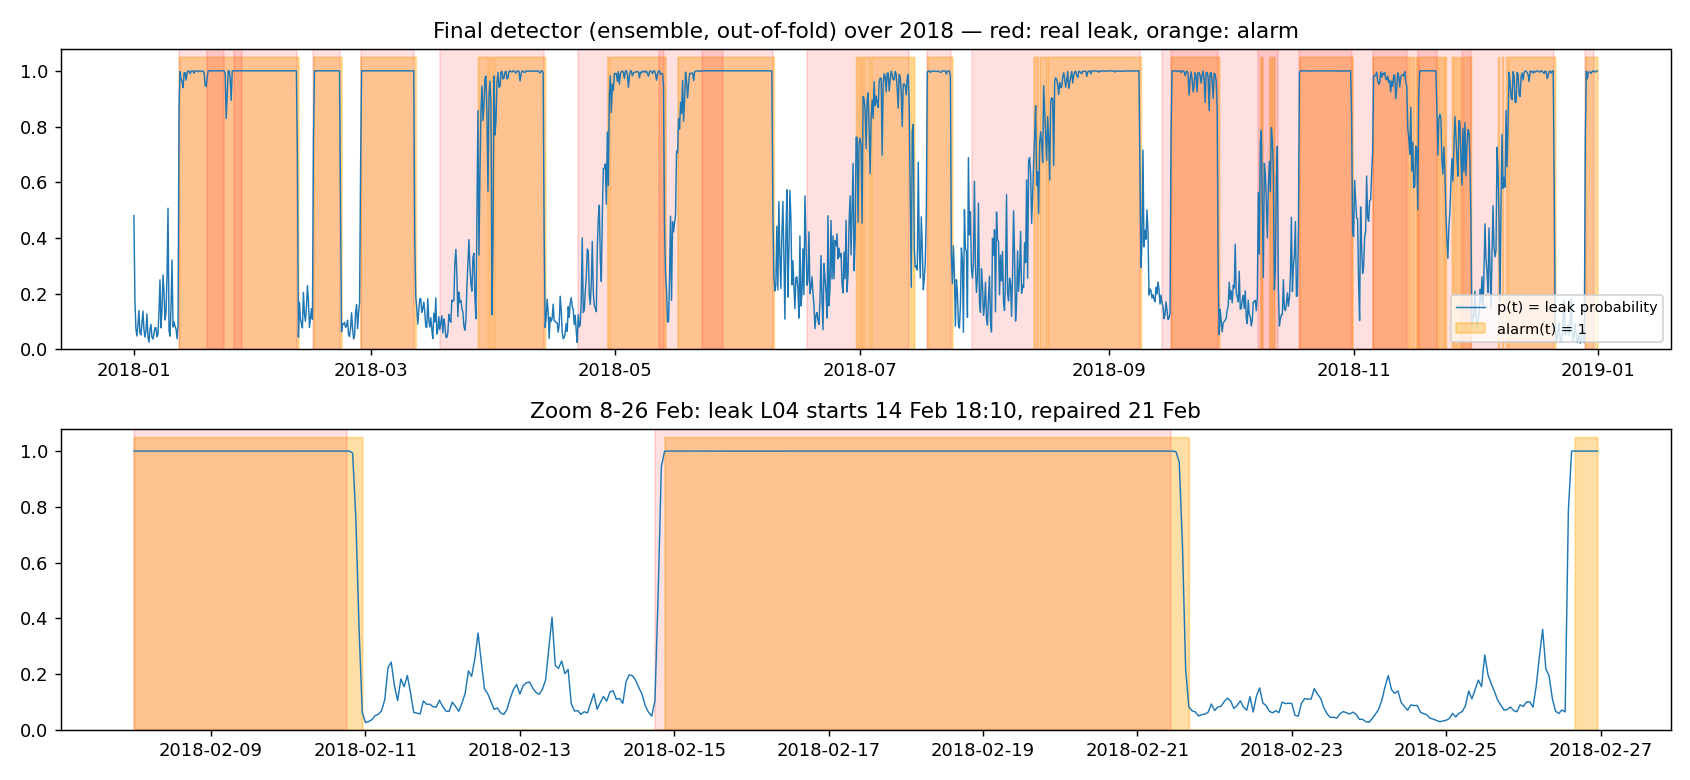
\includegraphics[width=\linewidth,trim=0 216bp 0 0,clip]{../outputs/part5/fig_detector_output.png}
  \end{center}
  \small خط آبی احتمال نشتِ مدل است. زمینهٔ قرمز زمانِ نشت واقعی و زمینهٔ نارنجی زمانِ روشن بودن هشدار را نشان می‌دهد. هم‌پوشانی این دو رنگ یعنی هشدار هنگام نشت فعال بوده است.
\end{frame}

\begin{frame}{نمودار زمانی آشکارساز: نمونهٔ فوریه}
  \begin{center}
  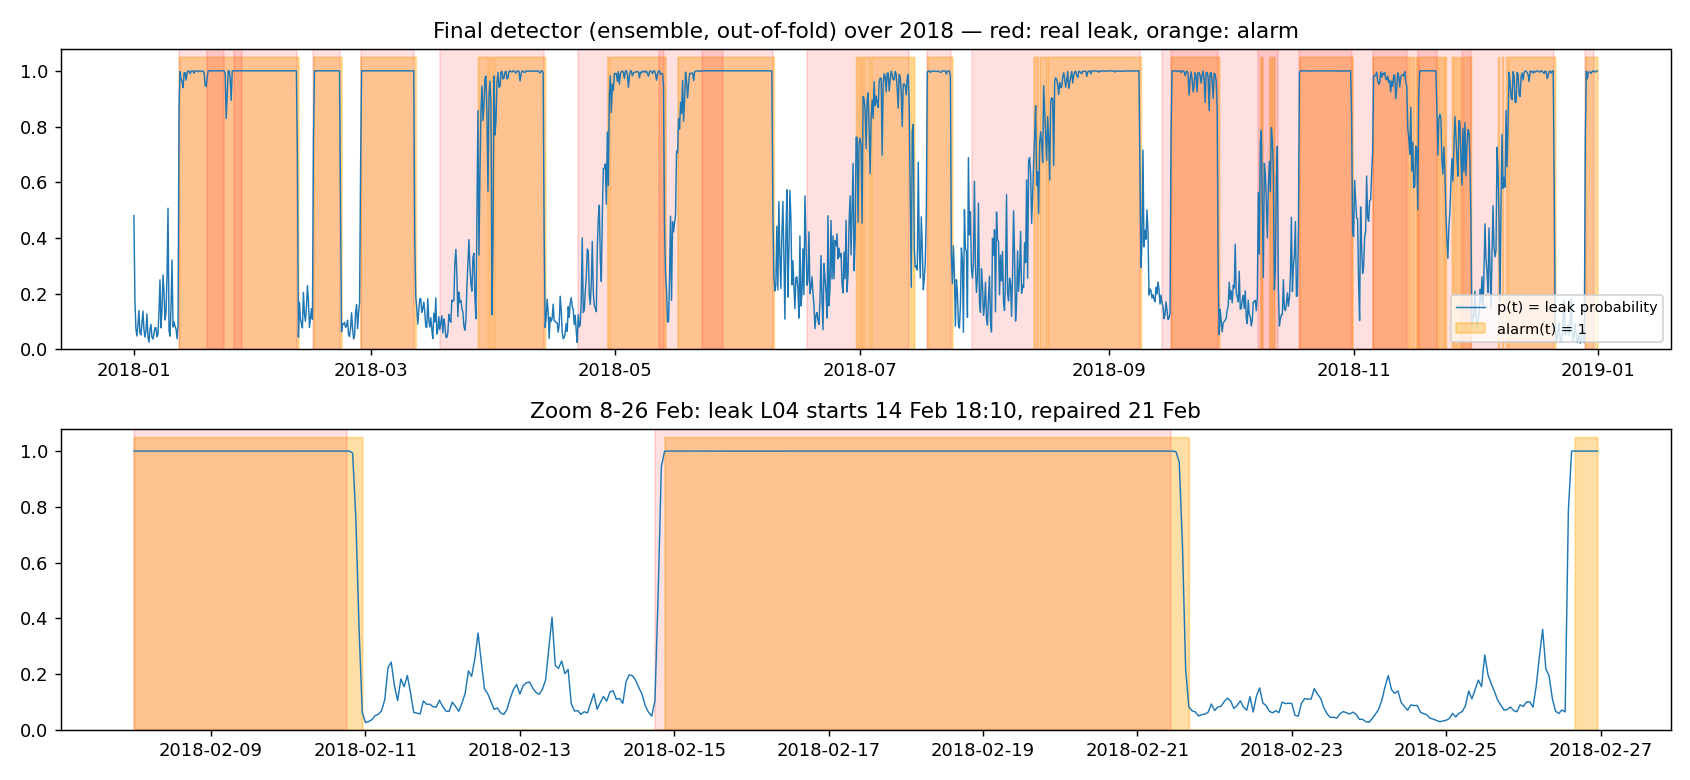
\includegraphics[width=\linewidth,trim=0 0 0 216bp,clip]{../outputs/part5/fig_detector_output.png}
  \end{center}
  \small نشت \eng{L04} از ۱۴ فوریه شروع شد و ۲۱ فوریه تعمیر شد. بالا رفتن خط آبی پس از شروع نشت و روشن شدن زمینهٔ نارنجی، روند تبدیل احتمال به هشدار را در یک بازهٔ کوتاه نشان می‌دهد.
\end{frame}

\begin{frame}{ورودی و برچسب مکان‌یاب}
  \begin{itemize}
  \item برای هر حسگر، اختلاف فشار از حالت عادی را در \key{۶ و ۲۴ ساعت گذشته} میانگین می‌گیریم: دو بردار ۳۳تایی.
  \item از هر بردار، میانگین حسگرها کم و سپس طول بردار به ۱ تبدیل می‌شود؛ \key{شکل افت فشار} برجسته می‌شود.
  \item لگاریتم بزرگیِ هر بردار پیش از نرمال‌سازی هم نگه داشته می‌شود: ۲ عدد. میانگین ۲۴ساعتهٔ اختلاف جریان: ۱ عدد.
  \end{itemize}
  \begin{center}\Large\color{navy}$2\times 33+2+1=\mathbf{69}$ ویژگی\end{center}
  \begin{block}{کدام ردیف‌ها برچسب قطعی دارند؟}
  برای آموزش واقعی فقط زمان‌هایی استفاده شد که دقیقاً یک نشت فعال بود و جریان آن دست‌کم ۲ مترمکعب‌برساعت بود. ارزیابی همچنان روی همهٔ ۲۰ رخداد انجام شد.
  \end{block}
\end{frame}

\begin{frame}{آموزش و ارزیابی مکان‌یاب}
  \begin{itemize}
  \item \eng{MLP}: ورودی ۶۹، دو لایهٔ پنهان ۱۲۸ و ۶۴، خروجی \eng{softmax} برای ۲۰ خوشه.
  \item \eng{BatchNorm}، \eng{ReLU} و \eng{Dropout(0.3)}؛ \eng{Adam} با نرخ ۰٫۰۰۱، وزن‌کاهی ۰٫۰۰۰۱، ۱۵ دوره، دستهٔ ۵۱۲تایی.
  \item دادهٔ آموزش: نمونهٔ واقعی + ۱۲ نسخهٔ مصنوعی؛ پنج \eng{seed} و میانگین احتمال خوشه‌ها.
  \item \key{تلاش جست‌وجو}: سهم لوله‌هایی که تا رسیدن به خوشهٔ درست باید بررسی شوند؛ کمتر بهتر.
  \item \key{دقت انتخاب اول}: سهم زمان‌های هشدار که خوشهٔ اول درست است؛ بیشتر بهتر.
  \end{itemize}
  \begin{block}{نکتهٔ معیار}
  هر معیار ابتدا برای هر نشت جداگانه حساب می‌شود و سپس میانگین ۲۰ نشت گرفته می‌شود تا نشت طولانی‌تر وزن بیشتری نگیرد.
  \end{block}
\end{frame}

\begin{frame}{مکان‌یاب چه‌قدر جست‌وجو را کم کرد؟}
  \begin{center}
  \begin{tabular}{r|c|c}
  روش & تلاش جست‌وجو $\downarrow$ & دقت انتخاب اول $\uparrow$\\\hline
  اولویت بر اساس تعداد لوله & ۰٫۵۵۴ & ۰٫۲۰۰\\
  نزدیک‌ترین امضای شبیه‌سازی‌شده & ۰٫۲۱۹ & ۰٫۵۷۱\\
  \eng{MLP} فقط با نشت مصنوعی & ۰٫۱۳۷ & ۰٫۷۸۴\\
  \textbf{\eng{MLP} واقعی + مصنوعی} & \textbf{۰٫۱۳۰} & \textbf{۰٫۸۰۰}
  \end{tabular}
  \end{center}
  \begin{itemize}
  \item تلاش ۰٫۱۳۰ یعنی تا رسیدن به خوشهٔ درست، به‌طور متوسط حدود \key{۱۱۸ لوله از ۹۰۵ لوله} بررسی می‌شوند.
  \item در آزمایش پنج‌باره، افزودن پنجرهٔ ۱ساعته یا شبکهٔ عمیق‌تر بهبود پایداری نداد.
  \item ۱۲ نسخهٔ مصنوعی، دقت انتخاب اول را نسبت به ۶ نسخه از ۷۴٫۲٪ به ۷۷٫۶٪ رساند؛ اختلاف اجراها هنوز مهم است.
  \end{itemize}
\end{frame}

\begin{frame}{چرا این دو طراحیِ مدل انتخاب شدند؟}
  \begin{block}{آشکارساز: \eng{AUROC} در پنج اجرای مستقل}
  \key{پنجرهٔ ۶ساعته، فقط دادهٔ واقعی: ۰٫۸۵۱}\\[0.2em]
  \key{همان ورودی + سه نسخهٔ مصنوعی: ۰٫۸۹۳ ± ۰٫۰۱۵}\\[0.3em]
  دادهٔ مصنوعی بهبود آشکاری داشت؛ پنجرهٔ ۶ساعته از ۱۲ساعته زودتر هشدار می‌داد.
  \end{block}
  \begin{block}{مکان‌یاب: دقت انتخاب اول در پنج اجرای مستقل}
  \key{واقعی + ۶ نسخهٔ مصنوعی: ۷۴٫۲٪}\\[0.2em]
  \key{واقعی + ۱۲ نسخهٔ مصنوعی: ۷۷٫۶٪}\\[0.3em]
  پنجرهٔ اضافه و شبکهٔ عمیق‌تر حدود ۷۴٪ بودند؛ بهبودِ اجرای تکیِ آن‌ها در تکرارها پایدار نماند.
  \end{block}
  \small معیار انتخاب، نتیجهٔ چهار بلوک \eng{OOF} و پایداری در چند \eng{seed} بود. پس از انتخاب طرح، احتمال‌های پنج مدل برای خروجی نهایی میانگین گرفته شدند.
\end{frame}

\begin{frame}{آیا امضای شبیه‌سازی به نشت واقعی شبیه است؟}
  \begin{columns}[T,onlytextwidth]
  \begin{column}{0.52\textwidth}
  \begin{itemize}
  \item شکل افت فشارِ اندازه‌گیری‌شده با امضای شبیه‌سازی‌شدهٔ همان محل مقایسه شد.
  \item ۱۸ نشت از ۲۰ نشت ساعت‌های مناسب برای این مقایسه داشتند.
  \item میانهٔ شباهت کسینوسی \key{۰٫۹۸۸}؛ ۱۵ مورد از ۱۸ مورد از حد ۰٫۷ گذشتند.
  \item خوشهٔ واقعی در ۱۳ مورد رتبهٔ اول و در ۱۶ مورد میان سه رتبهٔ اول بود.
  \item اندازهٔ افت همیشه دقیق درنمی‌آید؛ نسبت اندازهٔ مشاهده به شبیه‌سازی میانهٔ ۱٫۳۷ داشت.
  \end{itemize}
  \end{column}
  \begin{column}{0.45\textwidth}
  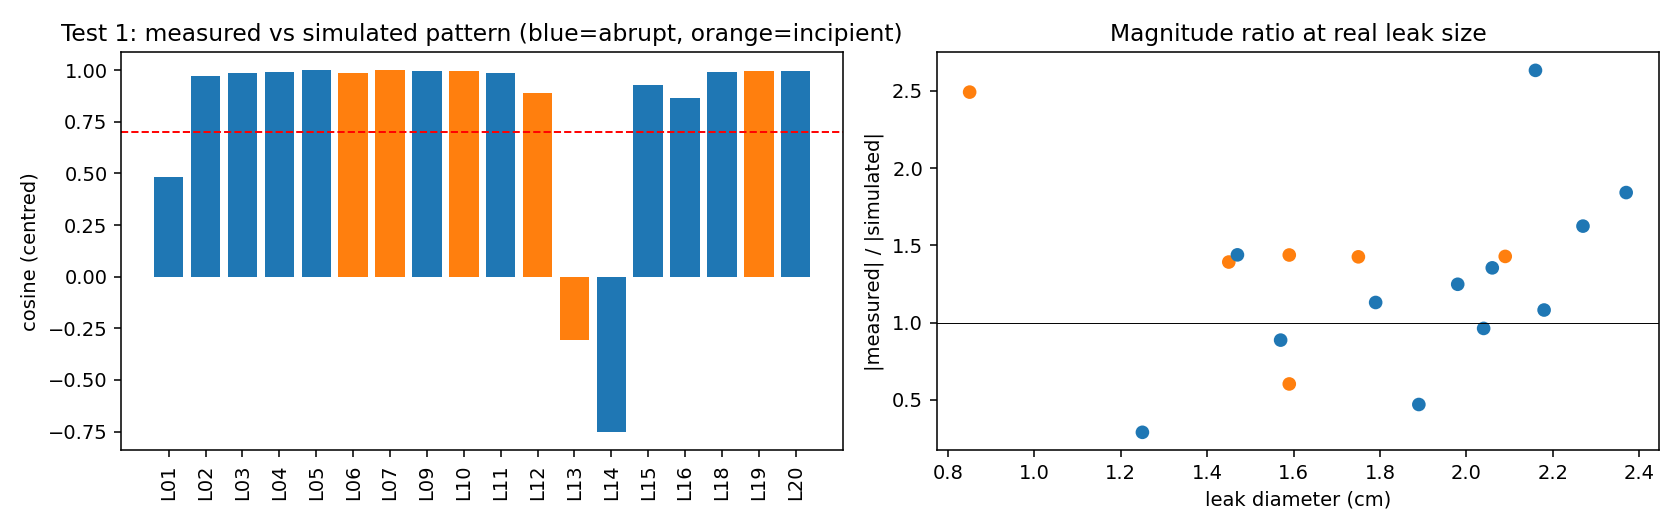
\includegraphics[width=\linewidth]{../outputs/part4/test1_cosine.png}
  \smallsource{outputs/part4/test1_cosine.png}
  \end{column}
  \end{columns}
\end{frame}

\begin{frame}{اجرای نهایی: آموزش، ذخیره، پیش‌بینی}
  \begin{enumerate}
  \item \eng{part5/train\_final.py} مدل رفتار عادی و پنج آشکارساز و پنج مکان‌یاب را با دادهٔ ۲۰۱۸ آموزش و ذخیره می‌کند.
  \item \eng{predict.py} چهار فایل حسگرِ بدون برچسب را می‌خواند و همان پیش‌پردازشِ ذخیره‌شده را اجرا می‌کند.
  \item میانگین پنج آشکارساز $\longrightarrow$ احتمال نشت $\longrightarrow$ قانون هشدارِ ثابت.
  \item فقط هنگام هشدار، میانگین پنج مکان‌یاب احتمال ۲۰ خوشه را می‌دهد.
  \end{enumerate}
  \begin{block}{خروجی و زمان اجرا}
  هر ردیف خروجی شامل \eng{Timestamp, p\_leak, alarm, c0...c19} است. پیش‌بینی یک سال کاملِ ۱۰۵٬۱۲۰ ردیفی روی \eng{CPU} حدود ۶٫۳ ثانیه طول کشید.
  \end{block}
\end{frame}

\begin{frame}{عدم‌قطعیت و محدودیت نتیجه}
  \begin{itemize}
  \item نتیجه‌های اصلی از پیش‌بینی \eng{OOF} سال ۲۰۱۸ آمده‌اند؛ دادهٔ مستقلِ سال بعد برای آزمون نداریم.
  \item بازهٔ ۹۰٪ بازنمونه‌گیری: \eng{AUROC} حدود \key{۰٫۸۷۶ تا ۰٫۹۱۶}؛ تلاش جست‌وجو حدود \key{۰٫۱۰ تا ۰٫۱۶}.
  \item بلوک تابستان سخت‌تر بود: \eng{AUROC} حدود \key{۰٫۷۷۱} و بعضی نشت‌های تدریجی بسیار دیر هشدار گرفتند.
  \item قاعدهٔ هشدار و طراحی مدل با همین خروجی‌های \eng{OOF} انتخاب شده‌اند؛ نتیجه ممکن است برای دادهٔ تازه خوش‌بینانه باشد.
  \item مکان‌یاب خوشه می‌دهد؛ اندازهٔ خوشه‌ها یکسان نیست و در بعضی موارد جست‌وجوی دستی همچنان زیاد است.
  \end{itemize}
  \begin{block}{جمع‌بندی}
  مدل هیدرولیکی نمونهٔ آموزشی و امضا می‌سازد؛ \eng{MLP}ها با دادهٔ واقعی و مصنوعی نشت را هشدار می‌دهند و جست‌وجو را به خوشه‌های محتمل محدود می‌کنند.
  \end{block}
\end{frame}

\end{document}
